\section{Extensión Temporal}
Estaba previsto que este proyecto tuviera una duración de 450 horas. Este valor surge a partir de un cálculo realizado a partir de los créditos obtenidos al acabar el TFG. Hemos supuesto una dedicación de 25 horas por crédito. Puesto que son 18 créditos, eso hace un total de 450 horas. Hemos realizado esta suposición basándonos en la dedicación de horas de otras asignaturas, otros proyectos de temática similar como \cite{wow-upc} \cite{netlogo} y las estimaciones dadas por la FIB (Facultad de Informática de Barcelona)\cite{fib_tfg}. Aunque hubo cierta búsqueda e investigación previa para acordar los datos básicos del TFG, podemos considerar que el desarrollo comenzó el día 21 de febrero de 2022 con la sesión informativa de GEP.   

Puesto que el turno de lectura de junio de 2022 comienza el día 27 \cite{fib_tfg} como podemos ver en la Figura \ref{fig:fechas}, el proyecto tiene como fecha límite máxima una semana antes, día 20 de junio de 2022. Si prevemos una dedicación diaria media de 4 horas, calculando a partir del día del inicio del TFG, disponemos de 476 horas aproximadamente hasta esta fecha. Con estas condiciones podemos estimar que el trabajo se encuentre completamente finalizado el día 14 de junio de 2022. Esta fecha es demasiado cercana a la fecha de límite de entrega, por lo tanto creemos que será necesaria una dedicación superior sobre todo los fines de semana.  
\begin{figure}[h]
    \centering
    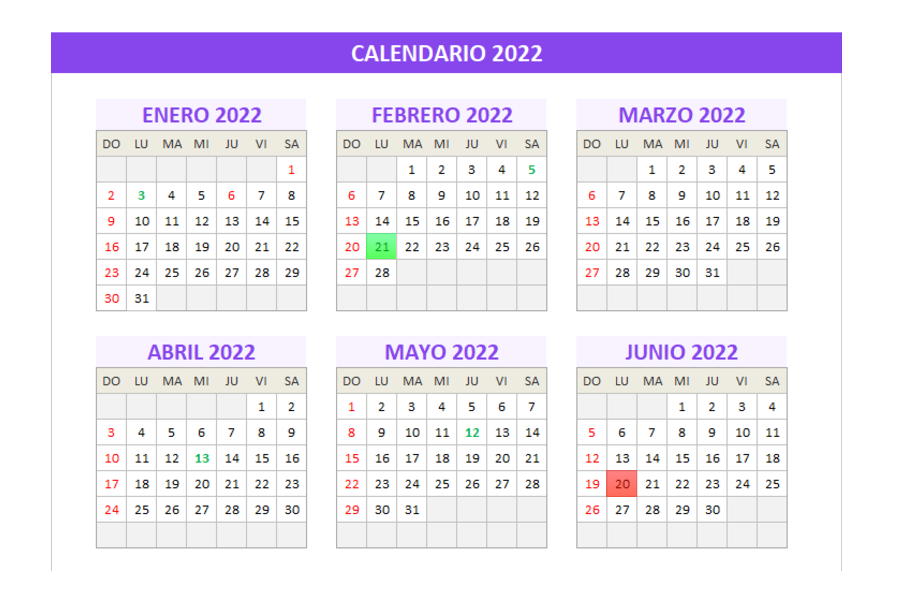
\includegraphics[width=0.5\textwidth]{img/fechas.png}
    \caption{Calendario del tiempo del trabajo. La fecha señalada en verde simboliza el inicio del trabajo y la fecha en rojo el día límite. [Elaboración propia]}
    \label{fig:fechas}
\end{figure}

Por ello, se dedicarán 2 horas adicionales sábados y domingos, asumiendo una dedicación de 4 horas de lunes a viernes y de 6 horas los fines de semana. Con esta nueva estimación, disponemos de 17 semanas hasta la fecha límite, lo que hace un total de 544 horas aproximadamente. En conclusión, suponiendo que no se presenta ningún contratiempo, el proyecto estaría finalizado por completo el día 31 de mayo de 2022. Esta fecha nos permite un gran margen de maniobra y aunque supone dedicación temporal considerable, sigue siendo una estimación más que razonable.


\section{Personal y material}
Para identificar el personal necesario para este proyecto nos hemos basado en los grandes grupos de tareas que distintas que contiene. En primer lugar está las tareas de definición del alcance, coordinación, toma de decisiones, etc. En segundo lugar están las tareas de análisis del estado del arte, creación de la documentación del proyecto, etc. Y finalmente las tareas de programación del entorno. Debido a este desglose de tareas, hemos decidido que serán necesarios 3 roles en el proyecto:
\begin{itemize}
    \item \textbf{Director del proyecto (D)}: Encargado de establecer el alcance del proyecto y sus características, desglose y asignación de tareas, control y seguimiento de estas y coordinación de los miembros del equipo.
    \item \textbf{Analista (A)}: Encargado de realizar una búsqueda y posterior análisis del estado del arte sobre los entornos multiagente con aspectos complejos y de escribir la documentación del proyecto y del entorno de manera que sea simple para otros investigadores usar esta tecnología.
    \item \textbf{Programador (P)}: Encargado de implementar y adaptar las características deseadas al entorno escogido o implementar uno desde 0 en caso de haberse decidido así. Además debe documentar el código escrito para facilitar su posible modificación en el futuro.  
\end{itemize}
 
 Una vez definido el personal, nos queda definir el material necesario para completar las tareas. Puesto que hay ciertas especificaciones del proyecto que aún deben decidirse, en este caso, cuál será el entorno y la tecnología que se usará, es posible que se necesite más material qué el especificado a continuación, por ejemplo licencias de uso de software, alquiler de servidores con capacidades de computación específicas, etc.
 El material (MAT) identificado como necesario es el siguiente:
 \begin{itemize}
     \item Tres ordenadores personales para los trabajadores.
     \item Un espacio de trabajo con internet.
     \item Como mínimo un servidor donde ejecutar el entrenamiento de los agentes.
 \end{itemize}
 
 Con respecto al software (SOFT), hemos identificado que se usará la herramienta de Git y GitLab para el control de versiones, Trello para el control de las tareas y LaTeX para la redacción de la documentación.